\documentclass[10pt,letterpaper]{article}

\usepackage{amsmath}
\usepackage{graphicx}

\newcommand{\sequence}[3]{#1$\rightarrow$#2$\rightarrow$#3}

\begin{document}

This is a test.  From \sequence{A}{B}{C} to \sequence{X}{Y}{Z}.

\section{Introduction}

Random noise is an important concept and is best described as a combination of random frequencies.  Take for example Figure~\ref{fig:exp_with_noise}.  Here we see random noise on an exponential.
%
\begin{figure}[!ht]
  \centering
  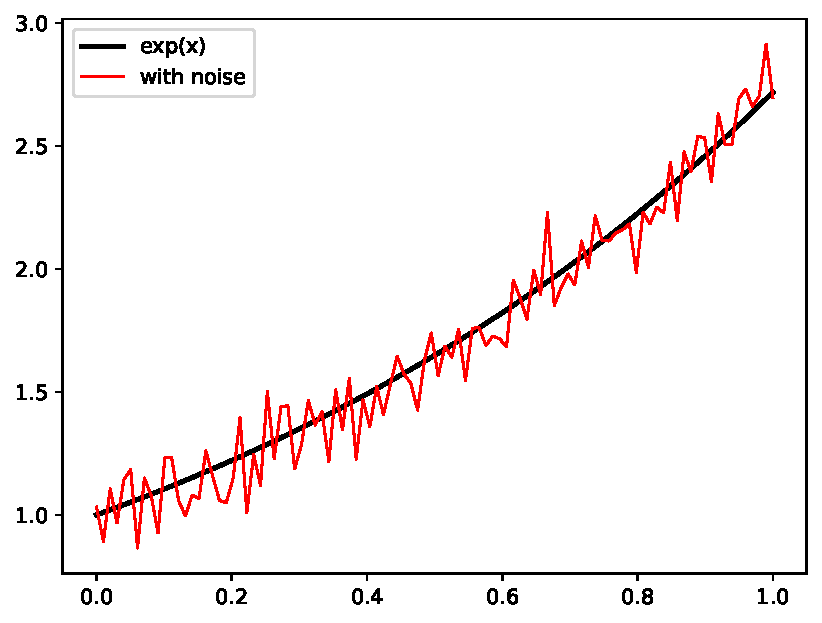
\includegraphics[width=0.5\textwidth]{./figures/exp_with_noise.pdf}
  \caption{An exponential function with random noise.}
  \label{fig:exp_with_noise}
\end{figure}

%
This is a reference to \cite{ChOlSe_2021_lsrbm}.

Sometimes, we wish to end a sentence with methods such as AMG.  However spacing can be slightly off.

\section{Background}
\section{Algorithm}
\section{Numerical Results}
\subsection{Experiment \# 1}
\subsection{Experiment \# 2}
% TODO did we have a third experiment?  If so add it.
\section{Conclusion}
% TODO add some comments on future work

\bibliographystyle{plain}
\bibliography{refs_example.bib}

% TODO add funding acknowledgements

\end{document}

